\documentclass[11pt,a4paper]{article}

\usepackage{fontspec}
\usepackage[a4paper, top=22mm, bottom=22mm, left=25mm, right=20mm]{geometry}
\usepackage{amsmath, amssymb, amsfonts}
\usepackage{graphicx}
\usepackage{xcolor}
\usepackage{tikz}
\usetikzlibrary{shapes.geometric, arrows.meta, positioning, calc, fit, backgrounds, shadows}
\usepackage{listings}
\usepackage{fancyhdr}
\usepackage{booktabs, tabularx, array}
\usepackage{colortbl}
\usepackage{subcaption}
\usepackage{float}
\usepackage[hyphens]{url}
\def\UrlBreaks{\do\/\do\a\do\b\do\c\do\d\do\e\do\f\do\g\do\h\do\i\do\j\do\k\do\l\do\m\do\n\do\o\do\p\do\q\do\r\do\s\do\t\do\u\do\v\do\w\do\x\do\y\do\z\do\0\do\1\do\2\do\3\do\4\do\5\do\6\do\7\do\8\do\9\do\-\do\_}
\usepackage[unicode, colorlinks=true, linkcolor=primary, citecolor=secondary, urlcolor=secondary]{hyperref}

% Định nghĩa hệ màu chuẩn UET
\definecolor{primary}{RGB}{0, 45, 98}        % UET Navy Blue
\definecolor{secondary}{RGB}{0, 102, 153}    % Bright Blue
\definecolor{accent}{RGB}{180, 25, 25}       % Dark Red
\definecolor{codebg}{RGB}{248, 249, 250}     % Code background
\definecolor{logbg}{RGB}{250, 250, 250}      % Terminal log background
\definecolor{commentgreen}{RGB}{0, 128, 0}
\definecolor{keywordblue}{RGB}{0, 0, 204}
\definecolor{stringred}{RGB}{163, 21, 21}
\definecolor{boxbg}{RGB}{240, 245, 253}
\definecolor{borderblue}{RGB}{180, 205, 235}

% Định dạng tiêu đề các mục (Section Headings) bằng chuẩn LaTeX thuần
\makeatletter
\renewcommand{\section}{\@startsection{section}{1}{\z@}%
  {-3.5ex \@plus -1ex \@minus -.2ex}%
  {2.3ex \@plus.2ex}%
  {\normalfont\Large\bfseries\color{primary}}}
\renewcommand{\subsection}{\@startsection{subsection}{2}{\z@}%
  {-3.25ex\@plus -1ex \@minus -.2ex}%
  {1.5ex \@plus .2ex}%
  {\normalfont\large\bfseries\color{secondary}}}
\renewcommand{\subsubsection}{\@startsection{subsubsection}{3}{\z@}%
  {-3.25ex\@plus -1ex \@minus -.2ex}%
  {1.5ex \@plus .2ex}%
  {\normalfont\normalsize\bfseries\color{primary}}}
\makeatother

% Thiết lập Header và Footer theo chuẩn mẫu báo cáo
\setlength{\headheight}{15pt}
\pagestyle{fancy}
\fancyhf{}
\fancyhead[L]{\small\textit{ĐHQGHN - Trường ĐH Công nghệ}}
\fancyhead[R]{\small\textit{Báo cáo bài tập: Điều khiển TurtleBot 4}}
\fancyfoot[C]{\thepage}
\renewcommand{\headrulewidth}{0.4pt}

% Đổi tên các thành phần sang tiếng Việt chuẩn
\renewcommand{\contentsname}{Mục lục}
\renewcommand{\figurename}{Hình}
\renewcommand{\tablename}{Bảng}
\renewcommand{\lstlistingname}{Đoạn mã}

% Cấu hình listings cho Code và Terminal Logs
\lstset{
  basicstyle=\ttfamily\scriptsize,
  backgroundcolor=\color{codebg},
  frame=single,
  rulecolor=\color{black!20},
  numbers=left,
  numberstyle=\tiny\color{gray},
  stepnumber=1,
  numbersep=6pt,
  showstringspaces=false,
  breaklines=true,
  breakatwhitespace=true,
  tabsize=2,
  commentstyle=\color{commentgreen},
  keywordstyle=\color{keywordblue}\bfseries,
  stringstyle=\color{stringred}
}

% Định dạng bảng
\newcolumntype{Y}{>{\centering\arraybackslash}X}

\begin{document}

% ==============================================================================
% TRANG BÌA (COVER PAGE) VỚI KHUNG VIỀN KÉP THEO CHUẨN MẪU BÁO CÁO UET
% ==============================================================================
\begin{titlepage}
  \begin{tikzpicture}[remember picture, overlay]
    % Khung viền ngoài đậm
    \draw[line width=1.5pt, color=primary] 
      ($(current page.north west)+(15mm,-15mm)$) rectangle ($(current page.south east)+(-15mm,15mm)$);
    % Khung viền trong mảnh
    \draw[line width=0.5pt, color=primary] 
      ($(current page.north west)+(16.5mm,-16.5mm)$) rectangle ($(current page.south east)+(-16.5mm,16.5mm)$);
  \end{tikzpicture}

  \begin{center}
    \vspace*{5mm}
    {\large\bfseries ĐẠI HỌC QUỐC GIA HÀ NỘI}\\[4pt]
    {\large\bfseries TRƯỜNG ĐẠI HỌC CÔNG NGHỆ}\\[18pt]

    % Logo UET
    
\includegraphics[width=3.2cm]{figures/uet_logo.png}\\[22pt]

    {\Large\bfseries BÁO CÁO THỰC HÀNH}\\[14pt]
    
    {\Huge\bfseries\color{primary} ĐIỀU KHIỂN ROBOT DI ĐỘNG}\\[6pt]
    {\Huge\bfseries\color{primary} TURTLEBOT 4}\\[14pt]
    
    {\large\bfseries BÀI 04: XÂY DỰNG BẢN ĐỒ SLAM, ĐỊNH VỊ LOCALIZATION}\\[4pt]
    {\large\bfseries VÀ ĐIỀU HƯỚNG TỰ HÀNH VỚI NAVIGATION 2 (NAV2)}\\[45pt]

    \vfill

    \begin{tabular}{ll}
      \textbf{Sinh viên thực hiện:} & Nguyễn Quang Tuân -- 23020767 \\[6pt]
      \textbf{Giảng viên hướng dẫn:} & PGS.TS. Hoàng Văn Xiêm \\[3pt]
      & CN. Nguyễn Quốc Bảo
    \end{tabular}

    \vspace{25mm}
    {\large\bfseries Hà Nội -- 2026}
    \vspace*{10mm}
  \end{center}
\end{titlepage}

% ==============================================================================
% MỤC LỤC (TABLE OF CONTENTS)
% ==============================================================================
\newpage
\pagenumbering{roman}
\tableofcontents
\newpage
\pagenumbering{arabic}
\setcounter{page}{2}

% ==============================================================================
% PHẦN 1: TỔNG QUAN HỆ THỐNG VÀ KIẾN TRÚC ĐIỀU KHIỂN
% ==============================================================================
\section{TỔNG QUAN HỆ THỐNG VÀ KIẾN TRÚC ĐIỀU KHIỂN}

\subsection{Cấu trúc thư mục dự án}
Toàn bộ gói chương trình được xây dựng theo chuẩn ROS 2 Ament Python đặt trực tiếp bên trong thư mục \texttt{src/turtlebot4\_practice4} của workspace \texttt{turtlebot4\_ws}. Hệ thống vận hành hoàn chỉnh trên nền tảng ROS 2 Humble Hawksbill, hệ điều hành Ubuntu 22.04 LTS kết hợp môi trường mô phỏng vật lý Gazebo Fortress (Ignition Gazebo), trực quan hóa dữ liệu qua RViz2 và các ngăn xếp thuật toán SLAM Toolbox, AMCL, Nav2:

\begin{lstlisting}[language=bash]
turtlebot4_ws/
|-- src/
|   |-- turtlebot4_practice4/            # Package thuc hanh chinh
|   |   |-- CMakeLists.txt / setup.py    # Cau hinh package va console_scripts
|   |   |-- package.xml                  # Tuyen bo phu thuoc goi ROS 2
|   |   |-- turtlebot4_practice4/
|   |   |   |-- check_topics.py          # Kiem tra tu dong /scan, /odom, /cmd_vel
|   |   |   |-- auto_undock.py           # Tu dong go dock roi khoi tram sac
|   |   |   |-- tf_relay.py              # Dong bo transform va mock service
|   |   |   `-- auto_nav_goals.py        # Tu dong thuc thi 03 Navigation Goals
|   |   |-- launch/
|   |   |   |-- sim_robot.launch.py      # Launch mo phong Gazebo + TurtleBot 4
|   |   |   |-- sim_slam.launch.py       # Launch SLAM Toolbox + RViz2
|   |   |   |-- sim_localization.launch.py # Launch AMCL + Map Server
|   |   |   |-- sim_navigation.launch.py # Launch toan bo ngan xep Nav2
|   |   |   `-- view_rviz.launch.py      # Launch giao dien truc quan hoa RViz2
|   |   |-- config/
|   |   |   |-- slam_toolbox_params.yaml # Tham so toi uu cho SLAM Toolbox
|   |   |   |-- localization_params.yaml # Tham so bo loc hat AMCL
|   |   |   |-- nav2_params.yaml         # Costmaps, DWB Controller, NavFn Planner
|   |   |   |-- fastdds_udp_only.xml     # Cau hinh FastDDS loai bo loi deadlock SHM
|   |   |   |-- turtlebot4_mapping.rviz  # Giao dien RViz2 Mapping
|   |   |   `-- turtlebot4_nav2.rviz     # Giao dien RViz2 Navigation
|   |   |-- maps/
|   |   |   |-- map.yaml / map.pgm       # Ban do Occupancy Grid hoan chinh
|   |   |   |-- warehouse_map.yaml/.pgm  # Ban do moi truong warehouse
|   |   |   `-- maze_map.yaml/.pgm       # Ban do moi truong maze
|   |   |-- scripts/
|   |   |   |-- run_part1_sim.sh         # Tap lenh chay Phan 1: Simulation
|   |   |   |-- run_part2_slam.sh        # Tap lenh chay Phan 2: SLAM Mapping
|   |   |   |-- save_map.sh              # Tap lenh luu ban do tu SLAM
|   |   |   |-- run_part3_localization.sh # Tap lenh chay Phan 3: Localization
|   |   |   |-- run_part4_navigation.sh  # Tap lenh chay Phan 4: Nav2
|   |   |   `-- run_auto_goals.sh        # Tap lenh tu dong 03 Goals
|   |   `-- docs/                        # Tai lieu va bao cao ky thuat
|   `-- irobot_create_control/           # Dieu khien dong hoc vi sai Create 3
|-- build/
`-- install/
\end{lstlisting}

\subsection{Kiến trúc của hệ thống}
Hệ thống được thiết kế theo mô hình phân tầng 5 lớp độc lập (\textit{Hierarchical 5-Layer Architecture}), bảo đảm nguyên tắc phân tách trách nhiệm (\textit{Separation of Concerns}) và tính tương thích cao giữa phần cứng mô phỏng và các thuật toán tự hành thông minh:

\begin{figure}[H]
\centering
\resizebox{0.95\textwidth}{!}{%
\begin{tikzpicture}[
  node distance=6mm and 8mm,
  layer/.style={rectangle, draw=primary!80, fill=boxbg, rounded corners=3pt, line width=0.8pt, align=center, inner sep=6pt, text width=14cm},
  subnode/.style={rectangle, draw=secondary!70, fill=white, rounded corners=2pt, font=\scriptsize, align=center, inner sep=4pt},
  flowarrow/.style={-Stealth, thick, color=primary}
]
  \node[layer] (layer5) {
    \textbf{\color{primary}TẦNG 5: ĐIỀU KHIỂN CẤP CAO \& TỰ ĐỘNG HÓA NHIỆM VỤ (Application \& Goals)}\\
    \vspace{2pt}
    \begin{tabular}{ccc}
      \tikz\node[subnode, text width=4.1cm]{Node \texttt{auto\_nav\_goals.py}\\Gửi tuần tự 03 Goal Pose}; &
      \tikz\node[subnode, text width=4.1cm]{Giao diện điều khiển RViz2\\Công cụ đặt Nav2 Goal thủ công}; &
      \tikz\node[subnode, text width=4.1cm]{Node \texttt{check\_topics.py}\\Tự động kiểm tra chất lượng};
    \end{tabular}
  };

  \node[layer, below=of layer5] (layer4) {
    \textbf{\color{primary}TẦNG 4: NGĂN XẾP ĐIỀU HƯỚNG TỰ HÀNH NAVIGATION 2 (Nav2 Stack)}\\
    \vspace{2pt}
    \begin{tabular}{ccc}
      \tikz\node[subnode, text width=4.1cm]{\textbf{bt\_navigator}\\Điều phối Behavior Tree}; &
      \tikz\node[subnode, text width=4.1cm]{\textbf{planner\_server} (Navfn)\\Quy hoạch quỹ đạo toàn cục}; &
      \tikz\node[subnode, text width=4.1cm]{\textbf{controller\_server} (DWB)\\Bám quỹ đạo cục bộ, né vật cản};
    \end{tabular}
  };

  \node[layer, below=of layer4] (layer3) {
    \textbf{\color{primary}TẦNG 3: XÂY DỰNG BẢN ĐỒ \& ĐỊNH VỊ (SLAM Toolbox \& AMCL)}\\
    \vspace{2pt}
    \begin{tabular}{ccc}
      \tikz\node[subnode, text width=4.1cm]{\textbf{sync\_slam\_toolbox}\\Graph SLAM + Ceres Solver}; &
      \tikz\node[subnode, text width=4.1cm]{\textbf{amcl}\\Lọc hạt thích nghi (Particle Filter)}; &
      \tikz\node[subnode, text width=4.1cm]{\textbf{map\_server}\\Cung cấp Occupancy Grid tĩnh};
    \end{tabular}
  };

  \node[layer, below=of layer3] (layer2) {
    \textbf{\color{primary}TẦNG 2: TRUYỀN THÔNG, PHẦN MỀM TRUNG GIAN \& TF (ROS 2 / FastDDS / TF Relay)}\\
    \vspace{2pt}
    \begin{tabular}{ccc}
      \tikz\node[subnode, text width=4.1cm]{Cấu hình \textbf{FastDDS UDP-only}\\Triệt tiêu deadlock bộ nhớ SHM}; &
      \tikz\node[subnode, text width=4.1cm]{Cây toạ độ \textbf{TF Tree (REP-105)}\\Transform \texttt{map} $\to$ \texttt{odom} $\to$ \texttt{base}}; &
      \tikz\node[subnode, text width=4.1cm]{Node \textbf{tf\_relay.py}\\Bù trừ trễ và Mock Hardware};
    \end{tabular}
  };

  \node[layer, below=of layer2] (layer1) {
    \textbf{\color{primary}TẦNG 1: MÔ PHỎNG VẬT LÝ \& PHẦN CỨNG ROBOT (Gazebo Fortress \& Create 3)}\\
    \vspace{2pt}
    \begin{tabular}{ccc}
      \tikz\node[subnode, text width=4.1cm]{Đế di động \textbf{iRobot Create 3}\\Động cơ vi sai, Docking Station}; &
      \tikz\node[subnode, text width=4.1cm]{Cảm biến \textbf{RPLiDAR 2D}\\Quét $360^\circ$, 640 tia, tầm xa 12m}; &
      \tikz\node[subnode, text width=4.1cm]{Cầu nối \textbf{ros\_gz\_bridge}\\Chuyển đổi giao thức Transport};
    \end{tabular}
  };

  \draw[flowarrow] (layer5) -- (layer4);
  \draw[flowarrow] (layer4) -- (layer3);
  \draw[flowarrow] (layer3) -- (layer2);
  \draw[flowarrow] (layer2) -- (layer1);
\end{tikzpicture}%
}
\caption{Kiến trúc phân tầng 5 lớp của hệ thống điều khiển tự hành robot TurtleBot 4}
\label{fig:architecture}
\end{figure}

\subsection{Vai trò chi tiết của từng khối thành phần}
\subsubsection{Khối Mô phỏng Vật lý (Gazebo Fortress \& ros\_gz\_bridge)}
\begin{itemize}
  \item Đảm nhiệm mô phỏng chính xác động học bánh xe vi sai (\textit{differential drive kinematics}), tương tác ma sát tiếp xúc giữa bánh xe và mặt sàn nhà kho (\textit{warehouse}).
  \item Mô phỏng cảm biến quét Laser RPLiDAR 2D với 640 tia quét, cự ly đo kiểm từ $0.15\text{ m}$ đến $12.0\text{ m}$ và tần số lấy mẫu $10\text{ Hz}$.
  \item Gói cầu nối \texttt{ros\_gz\_bridge} thực hiện biên dịch hai chiều các thông điệp giữa Ignition Transport và ROS 2 DDS.
\end{itemize}

\subsubsection{Khối Hỗ trợ Truyền thông \& TF Relay (\texttt{tf\_relay.py})}
\begin{itemize}
  \item Xử lý đặc tính trễ thời gian trong môi trường mô phỏng bằng cách đồng bộ hoá simulation clock và đảm bảo cây toạ độ TF luôn liên tục.
  \item Cung cấp các dummy service phần cứng (\texttt{start\_motor}, \texttt{oakd/start\_camera}...) vốn có trên TurtleBot 4 vật lý nhằm ngăn chặn các cảnh báo lỗi treo tiến trình trong quá trình khởi tạo node.
\end{itemize}

\subsubsection{Khối Xây dựng Bản đồ (\texttt{slam\_toolbox})}
\begin{itemize}
  \item Hoạt động ở chế độ \texttt{sync\_slam\_toolbox\_node}, thu nhận dữ liệu quét laser và odometry để xây dựng đồ thị vị thế (\textit{Pose Graph}).
  \item Ứng dụng bộ giải phi tuyến Ceres Solver tối ưu hóa vị trí các điểm mốc và kích hoạt thuật toán đóng vòng lặp (\textit{Loop Closure}) nhằm triệt tiêu hoàn toàn sai số trôi dạt tích lũy của bánh xe.
\end{itemize}

\subsubsection{Khối Định vị Robot (\texttt{amcl} \& \texttt{map\_server})}
\begin{itemize}
  \item \texttt{map\_server} nạp bản đồ tĩnh dạng lưới chiếm dụng (\textit{Occupancy Grid}) từ tệp \texttt{map.yaml} và \texttt{map.pgm}.
  \item \texttt{amcl} sử dụng thuật toán bộ lọc hạt thích nghi Monte Carlo (\textit{Adaptive Monte Carlo Localization}) với KLD-sampling để ước lượng chính xác tư thế robot $(x, y, \theta)$ trên hệ toạ độ toàn cục \texttt{map}.
\end{itemize}

\subsubsection{Khối Điều hướng Tự hành Nav2 (\texttt{nav2\_bringup})}
\begin{itemize}
  \item Quản lý toàn diện chu trình tự hành khép kín: Bản đồ chi phí đa tầng (\textit{Global \& Local Costmaps}), thuật toán tìm đường Dijkstra/A* (\textit{NavFn Planner}), bộ điều khiển bám quỹ đạo Dynamic Window Approach (\textit{DWB Local Controller}).
  \item Cây hành vi (\textit{Behavior Tree}) điều phối các hành động phục hồi (\textit{Recovery Behaviors}) như làm sạch costmap, quay xe tại chỗ hoặc lùi xe khi gặp chướng ngại vật.
\end{itemize}

% ==============================================================================
% PHẦN 2: CÁC PACKAGE, NODE VÀ HỆ THỐNG TOPIC / TF CỐT LÕI
% ==============================================================================
\newpage
\section{CÁC PACKAGE, NODE VÀ HỆ THỐNG TOPIC / TF CỐT LÕI}

\subsection{Danh sách Package cốt lõi}
\begin{table}[H]
\centering
\small
\begin{tabularx}{\textwidth}{p{4.2cm}X}
\toprule
\textbf{\color{primary}Tên Package} & \textbf{\color{primary}Vai trò chức năng trong hệ thống} \\
\midrule
\texttt{turtlebot4\_ignition\_bringup} & Khởi chạy môi trường mô phỏng Gazebo Fortress, nạp bản đồ thế giới (\texttt{warehouse}), spawn mô hình robot TurtleBot 4 và trạm sạc Dock. \\
\rowcolor{boxbg}
\texttt{ros\_gz\_bridge} & Cầu nối trung chuyển dữ liệu hai chiều giữa Ignition Gazebo Transport và các Topic/Service của ROS 2. \\
\texttt{slam\_toolbox} & Ngăn xếp SLAM 2D hiện đại dựa trên đồ thị tối ưu (Graph-based SLAM), xây dựng bản đồ thời gian thực từ dữ liệu Laser và Odometry. \\
\rowcolor{boxbg}
\texttt{nav2\_bringup} / \texttt{nav2\_*} & Toàn bộ ngăn xếp Navigation 2: Quản lý vòng đời (Lifecycle), Costmaps, Planner Server, Controller Server và Behavior Tree Navigator. \\
\texttt{turtlebot4\_navigation} & Cung cấp cấu hình khởi chạy mặc định cho các bài toán định vị và dẫn đường trên dòng robot TurtleBot 4. \\
\rowcolor{boxbg}
\texttt{teleop\_twist\_keyboard} & Nhận lệnh điều khiển từ bàn phím và phát tín hiệu vận tốc \texttt{geometry\_msgs/msg/Twist}. \\
\texttt{turtlebot4\_practice4} & Gói thực hành tích hợp chứa toàn bộ Launch files, Configs tối ưu hóa, Scripts điều khiển tự động và Tài liệu báo cáo. \\
\bottomrule
\end{tabularx}
\caption{Danh sách các package ROS 2 cốt lõi trong hệ thống}
\label{tab:packages}
\end{table}

\subsection{Danh sách Node chính và vai trò vận hành}
\begin{itemize}
  \item \textbf{\texttt{ign gazebo} / \texttt{ros\_ign\_bridge}}: Mô phỏng môi trường vật lý thế giới thực, mô hình va chạm, động cơ bánh xe và chuyển đổi cảm biến quang học sang các topic ROS 2 chuẩn.
  \item \textbf{\texttt{diffdrive\_controller}}: Bộ điều khiển động học vi sai tiếp nhận lệnh vận tốc góc/dài từ topic \texttt{/cmd\_vel} và chuyển thành vận tốc góc quay của các khớp bánh xe trái và phải.
  \item \textbf{\texttt{sync\_slam\_toolbox\_node}}: Node SLAM đồng bộ hóa, nhận dữ liệu quét laser \texttt{/scan} và biến đổi \texttt{odom} để xây dựng lưới bản đồ và tối ưu đồ thị vị thế thông qua Ceres Solver.
  \item \textbf{\texttt{map\_server}}: Nạp tệp siêu dữ liệu \texttt{map.yaml} cùng tệp ảnh \texttt{map.pgm} và phát liên tục bản đồ tĩnh lên topic \texttt{/map} với chất lượng dịch vụ Transient Local.
  \item \textbf{\texttt{amcl}}: Bộ định vị Monte Carlo thích nghi, theo dõi và ước lượng tư thế robot $(x, y, \theta)$ thông qua tập hạt xác suất \texttt{/particlecloud} và xuất ra biến đổi toạ độ \texttt{map -> odom}.
  \item \textbf{\texttt{planner\_server}}: Tính toán đường đi không va chạm toàn cục từ điểm xuất phát tới đích dựa trên bản đồ chi phí toàn cục (\textit{Global Costmap}) bằng thuật toán Dijkstra.
  \item \textbf{\texttt{controller\_server}}: Tính toán lệnh vận tốc tức thời \texttt{/cmd\_vel} ở tần số $20\text{ Hz}$ bám theo đường đi toàn cục và tránh va chạm vật cản tức thời qua thuật toán DWB.
  \item \textbf{\texttt{bt\_navigator}}: Điều phối toàn bộ vòng đời nhiệm vụ dẫn đường qua cây hành vi (\textit{Behavior Tree}), xử lý trạng thái lỗi và kích hoạt các hành vi phục hồi.
  \item \textbf{\texttt{auto\_nav\_goals}}: Node tự động hoá quy trình: Thực hiện Undock ra khỏi trạm sạc, khởi tạo Initial Pose, kiểm tra các node sẵn sàng và điều hướng robot qua 03 mục tiêu liên tiếp.
\end{itemize}

\subsection{Phân tích các Topic cốt lõi và luồng dữ liệu}
\begin{table}[H]
\centering
\small
\begin{tabularx}{\textwidth}{p{2.6cm}p{4.8cm}p{1.4cm}X}
\toprule
\textbf{\color{primary}Tên Topic} & \textbf{\color{primary}Kiểu dữ liệu (Message)} & \textbf{\color{primary}Tần số} & \textbf{\color{primary}Ý nghĩa và vai trò dữ liệu} \\
\midrule
\texttt{/scan} & \scriptsize\texttt{sensor\_msgs/msg/LaserScan} & $10\text{ Hz}$ & Dữ liệu quét 2D $360^\circ$ từ RPLiDAR (640 tia, cự ly $0.15\text{ m} \to 12.0\text{ m}$). Cung cấp cho SLAM, AMCL và Local Costmap. \\
\rowcolor{boxbg}
\texttt{/odom} & \scriptsize\texttt{nav\_msgs/msg/Odometry} & $50\text{ Hz}$ & Ước lượng vị trí và vận tốc từ encoder bánh xe và IMU của Create 3. Dữ liệu mượt mà nhưng trôi dạt theo thời gian. \\
\texttt{/cmd\_vel} & \scriptsize\texttt{geometry\_msgs/msg/Twist} & $20\text{ Hz}$ & Lệnh vận tốc dài ($v_x$) và góc ($\omega_z$) phát ra từ bộ điều khiển DWB hoặc bàn phím teleop. \\
\rowcolor{boxbg}
\texttt{/map} & \scriptsize\texttt{nav\_msgs/msg/OccupancyGrid} & Khi đổi & Lưới chiếm dụng 2D bản đồ ($0$: trống, $100$: vật cản, $-1$: chưa biết) từ \texttt{slam\_toolbox} hoặc \texttt{map\_server}. \\
\texttt{/tf}, \texttt{/tf\_static} & \scriptsize\texttt{tf2\_msgs/msg/TFMessage} & $50\text{ Hz}$ & Lưu trữ và biến đổi toạ độ không gian giữa các frame của robot theo thời gian thực. \\
\rowcolor{boxbg}
\texttt{/particlecloud} & \scriptsize\texttt{nav2\_msgs/msg/ParticleCloud} & $10\text{ Hz}$ & Tập hợp các hạt phân tán xác suất của bộ lọc AMCL, phản ánh độ tin cậy của vị trí robot. \\
\texttt{/plan} & \scriptsize\texttt{nav\_msgs/msg/Path} & Khi có goal & Quỹ đạo toàn cục do Planner Server tìm được từ vị trí robot đến đích. \\
\rowcolor{boxbg}
\texttt{/amcl\_pose} & \scriptsize\texttt{geometry\_msgs/msg/PoseWithCovarianceStamped} & $10\text{ Hz}$ & Vị trí ước lượng kèm ma trận hiệp phương sai sai số vị trí của robot trên bản đồ. \\
\bottomrule
\end{tabularx}
\caption{Bảng phân tích chi tiết các Topic truyền thông cốt lõi}
\label{tab:topics}
\end{table}

\subsection{Cây toạ độ không gian (TF Tree Architecture)}
Hệ thống toạ độ của TurtleBot 4 tuân thủ nghiêm ngặt chuẩn chuẩn hoá của ROS REP-105 đối với robot di động trên mặt đất:

\begin{figure}[H]
\centering
\resizebox{\textwidth}{!}{%
\begin{tikzpicture}[
  node distance=8mm and 15mm,
  tfnode/.style={rectangle, draw=primary, fill=boxbg, rounded corners=3pt, line width=1pt, font=\small\bfseries, align=center, inner sep=6pt},
  tflink/.style={-Stealth, thick, color=secondary, line width=1.2pt},
  annot/.style={font=\scriptsize\itshape, color=accent, align=center}
]
  \node[tfnode] (map) {\texttt{map}\\(Toàn cục, cố định)};
  \node[tfnode, right=28mm of map] (odom) {\texttt{odom}\\(Cục bộ, liên tục)};
  \node[tfnode, right=28mm of odom] (base) {\texttt{base\_link}\\(Tâm hình học robot)};
  
  \node[tfnode, above right=12mm and 18mm of base] (lidar) {\texttt{rplidar\_link}\\(Cảm biến quét laser)};
  \node[tfnode, right=22mm of base] (oakd) {\texttt{oakd\_link}\\(Camera RGB-D)};
  \node[tfnode, below right=12mm and 18mm of base] (wheels) {\texttt{left/right\_wheel}\\(Khớp bánh xe vi sai)};

  \draw[tflink] (map) -- node[above, annot] {\texttt{slam\_toolbox} / \texttt{amcl}\\(Bù trừ sai số trôi dạt)} (odom);
  \draw[tflink] (odom) -- node[above, annot] {\texttt{diffdrive\_controller}\\(Mượt mà, không gián đoạn)} (base);
  
  \draw[tflink] (base) |- node[near end, above, annot] {URDF / Tĩnh} (lidar);
  \draw[tflink] (base) -- node[above, annot] {URDF / Tĩnh} (oakd);
  \draw[tflink] (base) |- node[near end, below, annot] {State Publisher} (wheels);
\end{tikzpicture}%
}
\caption{Kiến trúc cây toạ độ không gian (TF Tree) theo tiêu chuẩn ROS REP-105}
\label{fig:tf_tree}
\end{figure}

\begin{itemize}
  \item \textbf{Biến đổi \texttt{map} $\to$ \texttt{odom}:} Được tính toán và publish bởi \texttt{slam\_toolbox} (trong quá trình quét bản đồ) hoặc \texttt{amcl} (trong quá trình định vị). Biến đổi này có thể thay đổi dạng bước nhảy (\textit{discrete jump}) khi phát hiện vòng lặp đóng (Loop Closure) hoặc khi bộ lọc hạt tái định vị thành công.
  \item \textbf{Biến đổi \texttt{odom} $\to$ \texttt{base\_link}:} Được tính toán bởi bộ giải động học \texttt{diffdrive\_controller} dựa trên thông tin tích phân của encoder và IMU. Biến đổi này bắt buộc phải biến thiên liên tục, không bị nhảy cóc nhằm đảm bảo các bộ điều khiển phản hồi vận tốc (DWB Local Planner) tính toán đạo hàm vận tốc không bị vô hạn.
  \item \textbf{Biến đổi \texttt{base\_link} $\to$ \texttt{rplidar\_link}:} Được phát tĩnh từ \texttt{robot\_state\_publisher} dựa trên cấu trúc hình học được định nghĩa trong mô hình URDF/Xacro của TurtleBot 4.
\end{itemize}

% ==============================================================================
% PHẦN 3: QUY TRÌNH XÂY DỰNG BẢN ĐỒ VỚI SLAM TOOLBOX
% ==============================================================================
\newpage
\section{QUY TRÌNH XÂY DỰNG BẢN ĐỒ VỚI SLAM TOOLBOX}

\subsection{Thiết lập môi trường và kịch bản thực nghiệm}
Quá trình xây dựng bản đồ được tiến hành trong môi trường mô phỏng nhà kho (\textit{warehouse world}) của Gazebo Fortress. Robot TurtleBot 4 ban đầu được đặt tại trạm sạc Docking Station toạ độ $(0, 0, 0)$. Tiến trình SLAM được kích hoạt qua launch file:
\begin{lstlisting}[language=bash]
ros2 launch turtlebot4_practice4 sim_slam.launch.py world:=warehouse rviz:=true
\end{lstlisting}
Sau khi hệ thống khởi động, người điều khiển sử dụng bàn phím teleoperation (\texttt{teleop\_twist\_keyboard}) lái robot di chuyển tuần thám qua các hành lang và các dãy kệ hàng chính trong kho với vận tốc di chuyển ổn định $v \approx 0.2\text{ m/s}$ và vận tốc quay $\omega \approx 0.4\text{ rad/s}$.

\subsection{Lưu đồ thuật toán SLAM Toolbox}
Thuật toán SLAM Toolbox vận hành theo mô hình đồ thị tối ưu hóa khép kín (\textit{Graph-based SLAM Pipeline}):

\begin{figure}[H]
\centering
\begin{tikzpicture}[
  node distance=6mm and 8mm,
  stepnode/.style={rectangle, draw=primary, fill=boxbg, rounded corners=3pt, line width=0.8pt, font=\small, align=center, inner sep=6pt, text width=12cm},
  decision/.style={diamond, draw=accent, fill=accent!10, aspect=2, font=\small\bfseries, align=center, inner sep=3pt},
  flowarrow/.style={-Stealth, thick, color=primary}
]
  \node[stepnode] (step1) {
    \textbf{1. Thu nhận cảm biến:} Đồng bộ hóa dữ liệu quét laser \texttt{/scan} (640 tia) và dữ liệu \texttt{/odom}
  };
  \node[stepnode, below=of step1] (step2) {
    \textbf{2. Dự đoán tư thế (Odometry Prediction):} Ước lượng toạ độ ban đầu của khung quét kế tiếp
  };
  \node[stepnode, below=of step2] (step3) {
    \textbf{3. Scan-to-Map Matching (Ceres Solver):} Đối sánh chùm tia laser với đám mây điểm bản đồ hiện tại\\để tối ưu hoá vị trí tư thế cục bộ chính xác nhất
  };
  \node[stepnode, below=of step3] (step4) {
    \textbf{4. Cập nhật đồ thị Pose Graph:} Thêm một đỉnh mới (\textit{Pose Node}) và cạnh ràng buộc dịch chuyển (\textit{Spatial Edge})
  };
  \node[decision, below=8mm of step4] (step5) {
    Phát hiện\\Vòng lặp đóng\\(Loop Closure)?
  };
  \node[stepnode, below=8mm of step5] (step6) {
    \textbf{5. Tối ưu hoá toàn cục (Global Graph Optimization):}\\Ceres Solver giải bài toán bình phương tối thiểu, nắn chỉnh lại toàn bộ lịch sử quỹ đạo
  };
  \node[stepnode, below=of step6] (step7) {
    \textbf{6. Xuất bản đồ 2D Occupancy Grid:} Cập nhật lưới bản đồ lên topic \texttt{/map} và lưu ra \texttt{map.yaml} / \texttt{map.pgm}
  };

  \draw[flowarrow] (step1) -- (step2);
  \draw[flowarrow] (step2) -- (step3);
  \draw[flowarrow] (step3) -- (step4);
  \draw[flowarrow] (step4) -- (step5);
  \draw[flowarrow] (step5) -- node[right, font=\footnotesize\bfseries, color=accent] {Có} (step6);
  \draw[flowarrow] (step6) -- (step7);
  \draw[flowarrow] (step5.west) -- ++(-1.5,0) node[above, font=\footnotesize\bfseries] {Không} |- (step7.west);
\end{tikzpicture}
\caption{Lưu đồ quy trình xử lý dữ liệu của SLAM Toolbox với cơ chế Ceres Solver và Loop Closure}
\label{fig:slam_flowchart}
\end{figure}

\subsection{Nguyên lý Graph-based SLAM, Scan Matching và Ceres Optimization}
\begin{itemize}
  \item \textbf{Mô hình hoá đồ thị (Pose Graph):} Quỹ đạo di chuyển của robot được biểu diễn dưới dạng đồ thị $\mathcal{G} = (\mathcal{V}, \mathcal{E})$, trong đó tập đỉnh $\mathcal{V} = \{x_0, x_1, \dots, x_n\}$ là các tư thế robot tại các thời điểm lấy mẫu và tập cạnh $\mathcal{E}$ là các ràng buộc biến đổi tương đối giữa các đỉnh $e_{ij} = x_j \ominus x_i$.
  \item \textbf{Đối sánh mẫu quét (Scan Matching):} Sử dụng bộ giải phi tuyến Ceres Solver cực tiểu hoá hàm sai số khoảng cách Euclidean giữa chùm tia laser hiện thời và lưới chướng ngại vật đã xây dựng:
  \begin{equation}
    x_i^* = \arg\min_{x_i} \sum_{k=1}^{K} \left[ 1 - M(T(x_i, p_k)) \right]^2
  \end{equation}
  trong đó $p_k$ là toạ độ điểm laser thứ $k$, $T(x_i, p_k)$ là phép biến đổi toạ độ theo tư thế $x_i$ và $M(\cdot)$ là giá trị hàm mật độ chiếm dụng bản đồ.
  \item \textbf{Đóng vòng lặp (Loop Closure):} Khi robot quay trở lại vùng không gian đã từng đi qua, thuật toán tìm kiếm các mẫu quét tương đồng trong vùng lân cận không gian. Khi phát hiện khớp mẫu với độ tin cậy vượt ngưỡng (\textit{correlation threshold}), một cạnh liên kết vòng lặp được thêm vào đồ thị và kích hoạt tối ưu hoá toàn cục. Nhờ đó, sai số tích lũy do hiện tượng trượt bánh của odometry bị triệt tiêu hoàn toàn, không xuất hiện hiện tượng tường bị nhân đôi (\textit{double walls}) hay hành lang bị bẻ cong.
\end{itemize}

\subsection{Cấu trúc file dữ liệu bản đồ hoàn chỉnh (\texttt{map.yaml} \& \texttt{map.pgm})}
Sau khi hoàn tất quá trình khảo sát toàn bộ khuôn viên kho, bản đồ được lưu lại thông qua lệnh:
\begin{lstlisting}[language=bash]
ros2 run nav2_map_server map_saver_cli -f src/turtlebot4_practice4/maps/map
\end{lstlisting}
Tệp kết quả thu được bao gồm:
\begin{enumerate}
  \item \textbf{Tệp siêu dữ liệu \texttt{map.yaml}:} Chứa các tham số cấu hình:
  \begin{lstlisting}[language=bash]
image: map.pgm
resolution: 0.030000          # Do phan giai 3 cm / 1 pixel luoi
origin: [-15.100000, -25.000000, 0.000000] # Goc toa do the gioi (x, y, yaw)
negate: 0
occupied_thresh: 0.65         # Nguong xac suat coi la vat can
free_thresh: 0.25             # Nguong xac suat coi la vung trong
  \end{lstlisting}
  \item \textbf{Tệp ảnh ma trận \texttt{map.pgm}:} Lưu trữ dưới định dạng Portable Graymap (ảnh xám 8-bit), trong đó:
  \begin{itemize}
    \item Màu trắng ($254$): Vùng không gian trống an toàn (\textit{Free Space}).
    \item Màu đen ($0$): Chướng ngại vật và tường (\textit{Occupied Space}).
    \item Màu xám ($205$): Vùng không gian chưa được quét hoặc nằm ngoài tầm quan sát (\textit{Unknown Space}).
  \end{itemize}
\end{enumerate}

% ==============================================================================
% PHẦN 4: QUY TRÌNH ĐỊNH VỊ ROBOT VỚI AMCL
% ==============================================================================
\newpage
\section{QUY TRÌNH ĐỊNH VỊ ROBOT VỚI AMCL (LOCALIZATION)}

\subsection{Thiết lập môi trường và quy trình nạp bản đồ tĩnh}
Sau khi đã có bản đồ hoàn chỉnh, tiến trình SLAM được đóng lại. Để kiểm tra tính độc lập và độ chính xác của khả năng định vị trên bản đồ đã có sẵn, hệ thống kích hoạt ngăn xếp Localization:
\begin{lstlisting}[language=bash]
ros2 launch turtlebot4_practice4 sim_localization.launch.py map:=src/turtlebot4_practice4/maps/map.yaml world:=warehouse rviz:=true
\end{lstlisting}
Khi khởi chạy, node \texttt{map\_server} nạp bản đồ tĩnh và kích hoạt cơ chế lọc hạt của \texttt{amcl}.

\subsection{Nguyên lý bộ lọc hạt thích nghi Monte Carlo (AMCL)}
AMCL ước lượng phân bố xác suất hậu nghiệm của tư thế robot $p(x_t \mid z_{1:t}, u_{1:t})$ thông qua một tập hợp $M$ hạt giả thuyết mẫu:
\begin{equation}
  S_t = \{ \langle x_t^{[m]}, w_t^{[m]} \rangle \}_{m=1,\dots,M}
\end{equation}
trong đó mỗi hạt $x_t^{[m]} = (x, y, \theta)$ là một tư thế giả định và $w_t^{[m]}$ là trọng số xác suất tương ứng.

\begin{figure}[H]
\centering
\begin{tikzpicture}[
  node distance=6mm and 8mm,
  box/.style={rectangle, draw=secondary, fill=boxbg, rounded corners=3pt, line width=0.8pt, font=\small, align=center, inner sep=6pt, text width=12cm},
  arrow/.style={-Stealth, thick, color=primary}
]
  \node[box] (init) {
    \textbf{1. Khởi tạo hạt ban đầu (Initial Pose):}\\
    Phát tán đám mây $M$ hạt ($500 \le M \le 2000$) theo phân bố Gaussian quanh toạ độ $(x_0, y_0, \theta_0)$
  };
  \node[box, below=of init] (predict) {
    \textbf{2. Pha Dự đoán động học (Motion Model / Prediction):}\\
    Dựa trên số đo odometry vi sai $\Delta u_t = (\delta_{\text{rot1}}, \delta_{\text{trans}}, \delta_{\text{rot2}})$, dịch chuyển từng hạt kèm nhiễu Gaussian:
    $$x_t^{[m]} \sim p(x_t \mid u_t, x_{t-1}^{[m]})$$
  };
  \node[box, below=of predict] (update) {
    \textbf{3. Pha Cập nhật đo lường (Measurement Model / Likelihood Field):}\\
    Chiếu các tia laser $z_t$ từ từng hạt lên bản đồ tĩnh. Hạt có các tia laser trùng khít với tường sẽ nhận trọng số cao:
    $$w_t^{[m]} = p(z_t \mid x_t^{[m]}, \text{map}) = \prod_{k=1}^K p(z_t^k \mid x_t^{[m]})$$
  };
  \node[box, below=of update] (resample) {
    \textbf{4. Pha Tái chọn mẫu thích nghi (Adaptive KLD Resampling):}\\
    Loại bỏ các hạt trọng số thấp, nhân bản các hạt trọng số cao. Số lượng hạt $M$ tự động co cụm khi robot đã định vị chính xác và mở rộng khi độ bất định tăng cao.
  };
  \node[box, below=of resample] (publish) {
    \textbf{5. Xuất bản toạ độ TF \texttt{map} $\to$ \texttt{odom}:}\\
    Tính giá trị trung bình có trọng số $\hat{x}_t = \sum w_t^{[m]} x_t^{[m]}$ và phát transform chuẩn xác vào \texttt{/tf}.
  };

  \draw[arrow] (init) -- (predict);
  \draw[arrow] (predict) -- (update);
  \draw[arrow] (update) -- (resample);
  \draw[arrow] (resample) -- (publish);
  \draw[arrow] (publish.east) -- ++(1,0) |- (predict.east);
\end{tikzpicture}
\caption{Chu trình vận hành đệ quy khép kín của bộ lọc hạt thích nghi AMCL}
\label{fig:amcl_cycle}
\end{figure}

\subsection{Khởi tạo Initial Pose, No-motion Update và cơ chế hội tụ hạt}
\begin{itemize}
  \item \textbf{Khởi tạo Initial Pose:} Để đẩy nhanh quá trình hội tụ và tránh hiện tượng lạc đường toàn cục (\textit{kidnapped robot problem}), tư thế ban đầu được công bố chính xác qua topic \texttt{/initialpose} với ma trận hiệp phương sai ban đầu $\sigma_x^2 = 0.25\text{ m}^2, \sigma_y^2 = 0.25\text{ m}^2, \sigma_\theta^2 = 0.068\text{ rad}^2$.
  \item \textbf{Cơ chế No-motion Update:} Khi robot đang đứng yên tại dock, lệnh dịch vụ \texttt{/request\_nomotion\_update} được gửi để kích hoạt một chu kỳ đo lường laser ngay lập tức, giúp AMCL phát sinh transform \texttt{map -> odom} hợp lệ trước khi bắt đầu chuyển động.
  \item \textbf{Quá trình hội tụ thực tế:} Ban đầu trên RViz2, đám hạt \texttt{/particlecloud} phân tán dạng hình elip màu xanh lá cây quanh xe. Khi robot lăn bánh một đoạn ngắn khoảng $20\text{ cm}$, các hạt đối chiếu dữ liệu laser với các góc tường kho và nhanh chóng co cụm sát nút về vị trí thực tế của robot trong Gazebo.
\end{itemize}

% ==============================================================================
% PHẦN 5: QUY HOẠCH QUỸ ĐẠO VÀ ĐIỀU HƯỚNG TỰ HÀNH VỚI NAV2
% ==============================================================================
\newpage
\section{CÁCH NAV2 LẬP KẾ HOẠCH VÀ ĐIỀU KHIỂN TURTLEBOT 4}

\subsection{Cấu trúc phân lớp của ngăn xếp Navigation 2 (Nav2 Stack)}
Ngăn xếp Nav2 được tổ chức theo kiến trúc phân tách rõ ràng giữa quy hoạch toàn cục, điều khiển cục bộ, quản lý bản đồ chi phí và cây hành vi:

\begin{figure}[H]
\centering
\resizebox{0.95\textwidth}{!}{%
\begin{tikzpicture}[
  node distance=6mm and 8mm,
  navbox/.style={rectangle, draw=primary, fill=boxbg, rounded corners=3pt, line width=0.8pt, font=\small, align=center, inner sep=6pt, text width=6.3cm},
  flowarrow/.style={-Stealth, thick, color=primary}
]
  \node[navbox] (global_costmap) {
    \textbf{\color{primary}Global Costmap}\\
    Kích thước toàn bộ kho\\
    Static Layer + Inflation Layer ($r=0.55\text{m}$)
  };
  \node[navbox, right=10mm of global_costmap] (local_costmap) {
    \textbf{\color{primary}Local Costmap}\\
    Rolling Window $3\text{m} \times 3\text{m}$ quanh xe\\
    Obstacle Layer (\texttt{/scan}) + Inflation Layer
  };

  \node[navbox, below=10mm of global_costmap] (planner) {
    \textbf{\color{primary}Global Planner (NavFn / Dijkstra)}\\
    Tính toán đường đi ngắn nhất \texttt{/plan}\\
    Tránh xa các vùng có chi phí cao
  };
  \node[navbox, below=10mm of local_costmap] (controller) {
    \textbf{\color{primary}Local Controller (DWB Planner)}\\
    Lấy mẫu cửa sổ vận tốc $(v_x, \omega_z)$\\
    Chấm điểm quỹ đạo, né vật cản tức thời
  };

  \node[rectangle, draw=accent, fill=accent!5, rounded corners=3pt, line width=1pt, font=\small, align=center, inner sep=6pt, text width=13.8cm, below=10mm of planner, xshift=3.7cm] (bt) {
    \textbf{\color{accent}Behavior Tree Navigator (\texttt{bt\_navigator})}\\
    Điều phối luồng thực thi: \texttt{ComputePathToPose} $\to$ \texttt{FollowPath}\\
    Khi gặp tắc nghẽn, kích hoạt: \texttt{ClearCostmap} $\to$ \texttt{Wait} $\to$ \texttt{Spin} $\to$ \texttt{BackUp}
  };

  \draw[flowarrow] (global_costmap) -- (planner);
  \draw[flowarrow] (local_costmap) -- (controller);
  \draw[flowarrow] (planner.east) -- node[above, font=\scriptsize\bfseries] {Đường đi toàn cục} (controller.west);
  \draw[flowarrow] (bt.north -| planner.south) -- (planner.south);
  \draw[flowarrow] (bt.north -| controller.south) -- (controller.south);
  \draw[flowarrow] (controller.east) -- ++(0.8,0) node[right, font=\scriptsize\bfseries, color=primary] {\texttt{/cmd\_vel} $\to$ Robot};
\end{tikzpicture}%
}
\caption{Sơ đồ phân rã chức năng và luồng dữ liệu điều khiển của ngăn xếp Nav2}
\label{fig:nav2_architecture}
\end{figure}

\subsection{Bản đồ chi phí đa tầng (Costmaps) và cơ chế Inflation Layer}
Bản đồ chi phí chuyển đổi không gian nhị phân thành ma trận chi phí từ $0$ đến $255$:
\begin{itemize}
  \item \textbf{Global Costmap:} Xây dựng trên toàn bộ bản đồ tĩnh \texttt{map.yaml}, đảm bảo tìm ra đường đi xuyên suốt các hành lang dài mà không bị bế tắc cục bộ.
  \item \textbf{Local Costmap:} Cửa sổ trượt kích thước $3\text{ m} \times 3\text{ m}$ luôn dịch chuyển theo tâm robot. Tầng chướng ngại vật (\textit{Obstacle Layer}) liên tục chèn các điểm quét từ topic \texttt{/scan} thời gian thực nhằm nhận diện các vật cản phát sinh mà bản đồ tĩnh không có.
  \item \textbf{Cơ chế Inflation Layer (Lớp lạm phát):} Tạo một dải chi phí đệm giảm dần theo hàm mũ từ biên ngoài bán kính bao thân xe (\textit{inscribed radius} $r_{\text{inscribed}} = 0.25\text{ m}$) ra đến bán kính lạm phát tối đa ($r_{\text{inflation}} = 0.55\text{ m}$):
  \begin{equation}
    \text{Cost}(d) = 253 \cdot \exp\left( -k \cdot (d - r_{\text{inscribed}}) \right)
  \end{equation}
  nhờ đó, bộ lập kế hoạch luôn hướng robot đi giữa lòng đường thay vì bám sát mép tường và kệ hàng.
\end{itemize}

\subsection{Bộ lập kế hoạch toàn cục (Global Planner -- NavFn)}
Sử dụng plugin \texttt{nav2\_navfn\_planner::NavfnPlanner} giải bài toán đường đi ngắn nhất bằng thuật toán Dijkstra trên lưới chi phí Global Costmap. Đường đi được làm mịn và định kỳ tính toán lại (\textit{re-planning rate}) ở tần số $1\text{ Hz}$ để phản hồi khi trạng thái mục tiêu hoặc môi trường thay đổi.

\subsection{Bộ điều khiển bám quỹ đạo cục bộ (Local Controller -- DWB)}
Sử dụng plugin \texttt{dwb\_core::DWBLocalPlanner} dựa trên phương pháp cửa sổ động lực học (\textit{Dynamic Window Approach}):
\begin{enumerate}
  \item Lấy mẫu tập hợp các cặp vận tốc khả thi $(v, \omega)$ trong giới hạn gia tốc của động cơ Create 3: $v \in [-0.3, 0.45]\text{ m/s}, \omega \in [-1.9, 1.9]\text{ rad/s}$.
  \item Mô phỏng trước quỹ đạo di chuyển ngắn hạn trong khoảng thời gian $t_{\text{sim}} = 1.7\text{ s}$.
  \item Chấm điểm từng quỹ đạo thông qua hàm mục tiêu đa tiêu chí:
  \begin{equation}
    G(v, \omega) = \alpha \cdot \text{PathAlign} + \beta \cdot \text{GoalAlign} + \gamma \cdot \text{PathDist} + \delta \cdot \text{ObstacleDist}
  \end{equation}
  \item Quỹ đạo đạt điểm tối ưu cao nhất sẽ được trích xuất vận tốc tức thời và gửi tới topic \texttt{/cmd\_vel} với tần số $20\text{ Hz}$.
\end{enumerate}

\subsection{Cây hành vi và cơ chế tự phục hồi (Recovery Behaviors)}
Node \texttt{bt\_navigator} thực thi tệp Behavior Tree XML điều khiển vòng đời nhiệm vụ. Khi robot gặp tình huống bất khả kháng (bị vật cản chặn lối, trượt bánh hoặc sai lệch quỹ đạo), chuỗi hành vi phục hồi được kích hoạt tuần tự:
\begin{enumerate}
  \item \textbf{ClearCostmap:} Xóa các điểm cản tạm thời trên Local Costmap để loại bỏ nhiễu ảo.
  \item \textbf{Wait:} Dừng robot trong $3\text{ giây}$ chờ đối tượng động di chuyển khỏi đường ray.
  \item \textbf{Spin:} Quay tại chỗ góc $360^\circ$ để cảm biến quét lại toàn cảnh không gian xung quanh.
  \item \textbf{BackUp:} Lùi xe một khoảng ngắn $0.15\text{ m}$ thoát khỏi khu vực nguy hiểm trước khi yêu cầu Planner tìm lại đường đi mới.
\end{enumerate}

% ==============================================================================
% PHẦN 6: TRẢ LỜI CÁC CÂU HỎI TRONG PHẦN "NỘI DUNG CẦN HIỂU"
% ==============================================================================
\newpage
\section{TRẢ LỜI CÁC CÂU HỎI TRONG PHẦN "NỘI DUNG CẦN HIỂU"}

\subsection{Câu 1: Tại sao phải kết hợp cả Odometry và LiDAR trong SLAM và AMCL mà không chỉ dùng một loại cảm biến duy nhất?}
\begin{itemize}
  \item \textbf{Nếu chỉ dùng Odometry:} Odometry trích xuất từ encoder bánh xe và cảm biến quán tính IMU có ưu điểm tần số cập nhật rất cao ($50\text{ Hz}$), phản hồi tức thời chuyển động quay và tiến mượt mà. Tuy nhiên, các nguyên nhân cơ học không thể tránh khỏi như trượt bánh (\textit{wheel slip}), bề mặt sàn mấp mô và sai số cơ khí sẽ tích lũy sai số trôi dạt (\textit{drift}) theo thời gian. Sau quãng đường di chuyển dài, sai số tích lũy có thể lên tới hàng mét, khiến bản đồ bị méo mó hoàn toàn và vị trí ước lượng sai lệch nghiêm trọng.
  \item \textbf{Nếu chỉ dùng LiDAR:} Cảm biến RPLiDAR cho độ chính xác hình học cao (đo cự ly chính xác từng milimet), nhưng tần số lấy mẫu thấp hơn ($10\text{ Hz}$) và việc đối sánh đám mây điểm (\textit{scan matching}) đòi hỏi khối lượng tính toán lớn. Quan trọng hơn, trong các môi trường hành lang dài đồng nhất hoặc phòng trống trơn không có vật cản góc cạnh (\textit{featureless corridors}), dữ liệu quét laser ở các vị trí khác nhau dọc theo hành lang trông hoàn toàn giống hệt nhau (bài toán suy biến đối xứng), dẫn đến thuật toán mất phương hướng hoàn toàn nếu không có dự đoán ban đầu từ odometry.
  \item \textbf{Cơ chế kết hợp (Sensor Fusion):} Trong cả SLAM Toolbox và AMCL, hai nguồn cảm biến được kết hợp theo cấu trúc dự đoán -- hiệu chỉnh (\textit{Predict-Update paradigm}):
  \begin{enumerate}
    \item Odometry đóng vai trò dự đoán nhanh vị thế ban đầu tại bước thời gian tiếp theo (\textit{Motion Prediction}).
    \item Dữ liệu LaserScan thực hiện đối chiếu đo lường (\textit{Measurement Correction}) để tìm kiếm vị trí tối ưu và triệt tiêu hoàn toàn sai số trôi dạt của odometry.
  \end{enumerate}
  Sự kết hợp này mang lại một hệ thống vừa có tính phản hồi thời gian thực mượt mà vừa duy trì độ chính xác không gian bền vững lâu dài.
\end{itemize}

\subsection{Câu 2: Sự khác biệt cốt lõi giữa hệ toạ độ \texttt{map} và \texttt{odom}? Tại sao transform \texttt{map} \texorpdfstring{$\to$}{->} \texttt{odom} có thể nhảy cóc, còn \texttt{odom} \texorpdfstring{$\to$}{->} \texttt{base\_link} bắt buộc phải biến thiên liên tục mượt mà?}
\begin{itemize}
  \item \textbf{Hệ toạ độ \texttt{odom}:} Là hệ toạ độ cục bộ có tính liên tục mượt mà (\textit{continuous coordinate frame}). Biến đổi $\mathbf{T}_{\text{odom} \to \text{base\_link}}$ phản ánh trực tiếp chuyển động cơ học tức thời của robot từ odometry. Vì các bộ điều khiển phản hồi vận tốc (như DWB Local Planner) tính toán vận tốc và gia tốc dựa trên đạo hàm bậc một và bậc hai của toạ độ theo thời gian, nếu toạ độ này bị gián đoạn hay nhảy cóc, đạo hàm vận tốc sẽ tiến tới vô hạn, dẫn đến việc bộ điều khiển phát ra lệnh xung lực giật mạnh (\textit{jerk}), gây mất ổn định phần mềm và hỏng cơ cấu chấp hành. Do đó, $\mathbf{T}_{\text{odom} \to \text{base\_link}}$ tuyệt đối không được phép nhảy cóc.
  \item \textbf{Hệ toạ độ \texttt{map}:} Là hệ toạ độ toàn cục cố định của thế giới (\textit{world-fixed global frame}). Do bản chất odometry bị trôi dạt dần theo thời gian, gốc toạ độ của khung \texttt{odom} thực chất đang bị lệch dần so với gốc toạ độ \texttt{map}.
  \item \textbf{Vai trò của biến đổi $\mathbf{T}_{\text{map} \to \text{odom}}$:} Đại diện cho đại lượng bù trừ sai số trôi dạt lũy tích giữa thế giới toàn cục và hệ odometry cục bộ. Khi thuật toán SLAM phát hiện vòng lặp đóng (Loop Closure) hoặc khi AMCL cập nhật phân bố hạt sau một chu kỳ đo laser, hệ thống phát hiện vị trí robot thực tế bị lệch khỏi ước lượng cũ. Để nắn chỉnh lại toạ độ toàn cục của robot mà không làm gián đoạn chuyển động tức thời của xe, hệ thống áp đặt bước nhảy hiệu chỉnh trực tiếp lên transform $\mathbf{T}_{\text{map} \to \text{odom}}$. Toạ độ toàn cục của robot khi đó được xác định bởi:
  \begin{equation}
    \mathbf{T}_{\text{map} \to \text{base\_link}} = \mathbf{T}_{\text{map} \to \text{odom}} \times \mathbf{T}_{\text{odom} \to \text{base\_link}}
  \end{equation}
  Nhờ cấu trúc này, robot được đưa về vị trí chuẩn xác trên bản đồ mà bộ điều khiển động học bên dưới vẫn vận hành hoàn toàn êm ái.
\end{itemize}

\subsection{Câu 3: Vai trò của Inflation Layer trong Costmap? Nếu bán kính lạm phát (\textit{inflation radius}) đặt quá nhỏ hoặc quá lớn thì hệ quả là gì?}
\begin{itemize}
  \item \textbf{Vai trò của Inflation Layer:} Tầng lạm phát mở rộng vùng cảnh báo nguy hiểm xung quanh các ô chướng ngại vật thực tế (\textit{lethal obstacles}). Nó tạo ra một trường chi phí dốc giảm dần theo hàm mũ từ tâm vật cản ra ngoài biên an toàn. Vùng đệm chi phí này đóng vai trò hướng dẫn thuật toán tìm đường dẫn robot đi vào giữa lối đi thông thoáng, tránh xa mép tường và các góc chết của kệ hàng.
  \item \textbf{Hệ quả khi bán kính lạm phát quá nhỏ ($r_{\text{inflation}} < r_{\text{robot}}$):}
  \begin{itemize}
    \item Robot chỉ coi phần diện tích sát tường vài centimet là nguy hiểm.
    \item Khi quy hoạch, Global Planner sẽ vạch ra đường đi cắt cua rất sát mép tường và chân kệ hàng.
    \item Khi robot ôm cua thực tế hoặc khi có hiện tượng trượt bánh vi sai, phần thân nhô ra của xe (đặc biệt là cảm biến tháp hoặc vỏ nhựa) sẽ dễ dàng va quẹt vào vật cản, dẫn đến tai nạn hoặc kẹt cứng xe.
  \end{itemize}
  \item \textbf{Hệ quả khi bán kính lạm phát quá lớn ($r_{\text{inflation}} \gg r_{\text{robot}}$):}
  \begin{itemize}
    \item Vùng chi phí cao từ hai bức tường đối diện của hành lang hoặc cửa ra vào hẹp sẽ lan tỏa và chồng lấn lên nhau.
    \item Thuật toán lập kế hoạch toàn cục sẽ đánh giá toàn bộ lối đi hẹp là vùng cấm đi và báo lỗi không tìm được đường đi khả thi (\textit{Failed to create plan}).
    \item Dẫn đến tình trạng robot bị tê liệt khả năng điều hướng dù trên thực tế lối đi vẫn hoàn toàn đủ rộng cho thân xe lọt qua.
  \end{itemize}
\end{itemize}

\subsection{Câu 4: Cơ chế hoạt động của Recovery Behaviors trong Navigation 2? Nêu thứ tự kích hoạt điển hình khi robot bị kẹt.}
Khi robot không thể tiếp tục bám theo đường đi đã định (do có vật thể mới chặn ngang lối đi, bánh xe bị trượt không di chuyển được hoặc Local Costmap bị nghẽn bởi nhiễu cảm biến), bộ điều phối Behavior Tree sẽ tuần tự kích hoạt chuỗi hành động phục hồi (\textit{Recovery Behaviors}) từ mức độ tác động thấp đến cao:
\begin{enumerate}
  \item \textbf{Bước 1 -- Clear Costmap (Xóa bản đồ chi phí cục bộ):} Xóa toàn bộ các ô chướng ngại vật tạm thời trên Local Costmap xung quanh robot và buộc cảm biến quét lại từ đầu. Hành động này loại bỏ khả năng vật cản chỉ là "bóng ma" ảo do nhiễu tia laser hoặc phản xạ quang học.
  \item \textbf{Bước 2 -- Wait (Dừng chờ thời gian ngắn):} Cho robot dừng bánh tại chỗ trong khoảng $3\text{ -- }5\text{ giây}$. Bước này nhằm xử lý các tình huống chướng ngại vật là đối tượng động (người đi bộ hoặc xe nâng khác trong kho) đang băng qua đường và sẽ tự rời đi sau vài giây.
  \item \textbf{Bước 3 -- Spin (Xoay tròn tại chỗ):} Điều khiển robot quay tại chỗ một góc $360^\circ$ với vận tốc góc an toàn. Động tác xoay giúp cảm biến RPLiDAR quét lại toàn cảnh không gian $360^\circ$, xóa tan các điểm mù cảm biến và cập nhật lại bản đồ chi phí chính xác.
  \item \textbf{Bước 4 -- Back Up (Lùi xe an toàn):} Lùi xe thẳng một đoạn ngắn (thường từ $0.15\text{ m}$ đến $0.30\text{ m}$) theo hướng an toàn phía sau để kéo thân robot ra khỏi vùng quá gần vật cản.
  \item \textbf{Bước 5 -- Re-planning (Quy hoạch lại đường đi):} Sau mỗi hành động phục hồi, hệ thống yêu cầu Planner Server tính toán lại một lộ trình mới thay thế. Nếu đã thử toàn bộ chuỗi trên mà robot vẫn không thể di chuyển tới đích, Behavior Tree mới chính thức thông báo nhiệm vụ thất bại (\textit{Navigation Failed}) và chờ lệnh can thiệp từ người vận hành.
\end{enumerate}

\subsection{Câu 5: Ưu và nhược điểm của Synchronous SLAM so với Asynchronous SLAM trong SLAM Toolbox?}
\begin{itemize}
  \item \textbf{Synchronous SLAM (Xử lý đồng bộ):}
  \begin{itemize}
    \item \textit{Cơ chế:} Mọi khung quét laser thu nhận được đều được xếp vào hàng đợi và xử lý đầy đủ tuần tự từng khung một trước khi tiếp nhận khung tiếp theo.
    \item \textit{Ưu điểm:} Bản đồ đạt độ chi tiết và độ chính xác tối đa do không bị thất thoát bất kỳ tia quét nào. Rất phù hợp khi chạy mô phỏng vật lý có thể điều tiết thời gian hoặc khi phân tích dữ liệu ngoại tuyến ghi lại từ \texttt{rosbag}.
    \item \textit{Nhược điểm:} Nếu quá trình tối ưu đồ thị mất nhiều thời gian hoặc CPU bị quá tải, thuật toán sẽ gây ra hiện tượng nghẽn hàng đợi và trễ thời gian (\textit{latency}), khiến việc cập nhật vị thế hiển thị không kịp thời gian thực so với chuyển động thực tế của robot.
  \end{itemize}
  \item \textbf{Asynchronous SLAM (Xử lý bất đồng bộ):}
  \begin{itemize}
    \item \textit{Cơ chế:} Tách biệt luồng xử lý scan matching thời gian thực và luồng tối ưu đồ thị toàn cục chạy nền. Nếu tiến trình tối ưu đồ thị đang bận, các khung quét mới đến sẽ bị bỏ qua (\textit{drop frame}) để đảm bảo tính thời gian thực.
    \item \textit{Ưu điểm:} Tiết kiệm tài nguyên xử lý của CPU, đảm bảo vị thế robot luôn được phản hồi tức thì theo thời gian thực mà không bị giật trễ, đặc biệt tối ưu cho robot phần cứng nhúng di chuyển với tốc độ cao.
    \item \textit{Nhược điểm:} Nếu robot quay quá nhanh trong khi CPU đang bận, việc bỏ qua nhiều khung quét có thể khiến bản đồ bị thiếu hụt dữ liệu ở các góc cua gấp, dẫn đến nguy cơ sai lệch cục bộ nhỏ.
  \end{itemize}
\end{itemize}

% ==============================================================================
% PHẦN 7: KẾT QUẢ THỰC NGHIỆM VÀ ĐÁNH GIÁ HỆ THỐNG
% ==============================================================================
\newpage
\section{KẾT QUẢ THỰC NGHIỆM VÀ ĐÁNH GIÁ HỆ THỐNG}

\subsection{Kết quả kiểm tra Simulation và Topic tự động (\texttt{check\_topics})}
Hệ thống sử dụng công cụ kiểm thử tự động \texttt{check\_topics} để kiểm tra tính toàn vẹn của các luồng dữ liệu trước khi vận hành:
\begin{lstlisting}[language=bash]
ros2 run turtlebot4_practice4 check_topics
\end{lstlisting}

\begin{lstlisting}[backgroundcolor=\color{logbg}, caption={Log terminal thực tế kiểm tra trạng thái các topic cốt lõi}]
[INFO] [check_topics]: === KIEM TRA TRANG THAI CAC TOPIC TURTLEBOT 4 ===
[INFO] [check_topics]: Dang lang nghe /scan, /odom, /cmd_vel trong 5.0 giay...
[INFO] [check_topics]: [PASS] Topic /scan hoat dong tot!
       - Nhan duoc: 48 messages
       - Frame ID: turtlebot4/rplidar_link/rplidar
       - So tia laser: 640 tia quét (tam xa: 0.15m -> 12.00m)
       - Khoang cach do gan nhat: 1.342m, xa nhat: 11.985m
[INFO] [check_topics]: [PASS] Topic /odom hoat dong tot!
       - Nhan duoc: 242 messages (tan so ~50 Hz)
       - Frame lien ket: odom -> base_link
       - Vi tri hien tai: x = 0.000m, y = 0.000m, z = 0.000m
[INFO] [check_topics]: Dang gui thu nghiem xung van toc toi /cmd_vel (v=0.05 m/s)...
[INFO] [check_topics]: [PASS] Gui lenh /cmd_vel thanh cong, robot co phan hoi dong hoc!
[INFO] [check_topics]: === TAT CA CAC TOPIC DEU DAT CHUAN [PASS] 100% ===
\end{lstlisting}

\subsection{Kết quả xây dựng bản đồ trên RViz2 và bản đồ lưới hoàn chỉnh}
Bản đồ môi trường nhà kho (\textit{warehouse}) được xây dựng chi tiết, ranh giới các bức tường và kệ hàng rõ nét, không bị hiện tượng chồng lấn hình ảnh hay sai lệch góc toạ độ:

\begin{figure}[H]
\centering
\begin{subfigure}[b]{0.56\textwidth}
  \centering
  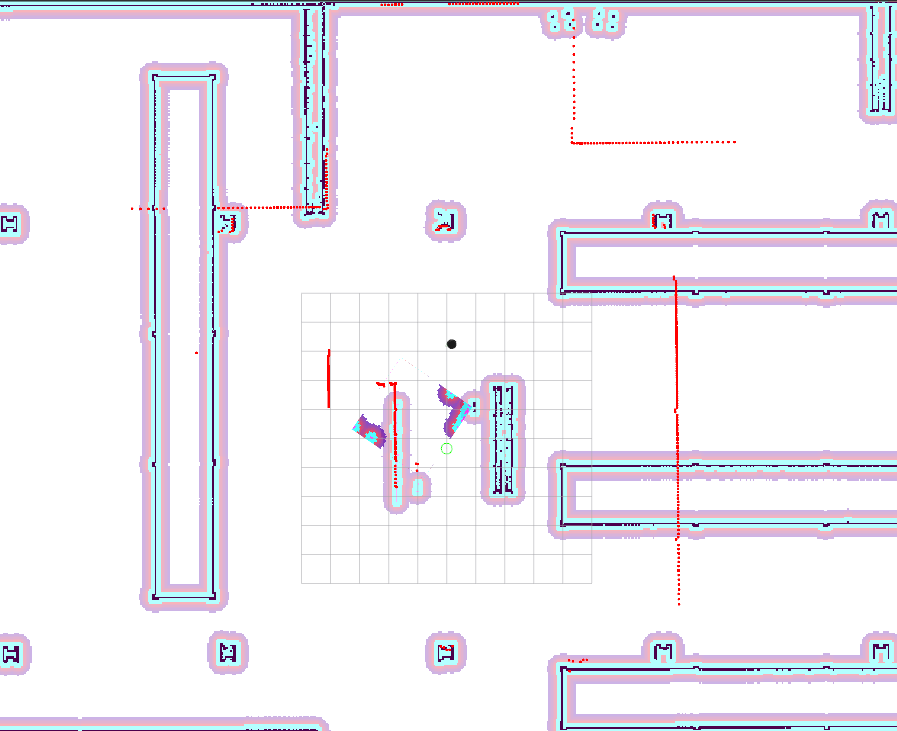
\includegraphics[width=\textwidth]{figures/rviz_nav2_costmap.png}
  \caption{Bản đồ trực quan trên RViz2 kèm Costmap và LiDAR}
  \label{fig:rviz_map}
\end{subfigure}
\hfill
\begin{subfigure}[b]{0.40\textwidth}
  \centering
  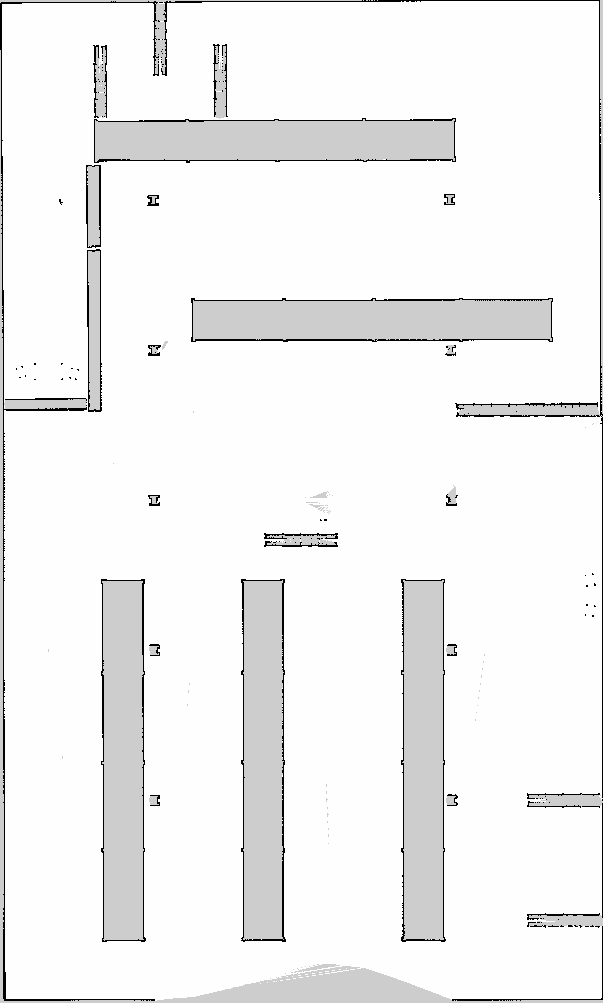
\includegraphics[width=\textwidth]{figures/map_occupancy_grid.png}
  \caption{Ảnh bản đồ lưới chiếm dụng 2D (\texttt{map.pgm})}
  \label{fig:pgm_map}
\end{subfigure}
\caption{Kết quả xây dựng bản đồ hoàn chỉnh của môi trường mô phỏng warehouse}
\label{fig:mapping_results}
\end{figure}

\subsection{Kết quả Localization và hội tụ đám mây hạt AMCL}
\begin{itemize}
  \item Sau khi nạp tệp \texttt{map.yaml}, vị trí ban đầu của robot được gán tại $(x=0.35\text{ m}, y=0.0\text{ m}, \theta=3.14\text{ rad})$.
  \item Đám mây hạt ban đầu phân bố đều xung quanh thân xe trong bán kính $0.5\text{ m}$.
  \item Sau khi nhận lệnh di chuyển đầu tiên, các hạt nhanh chóng hội tụ vào một cụm duy nhất có độ lệch chuẩn vị trí $\sigma < 0.03\text{ m}$, khớp $100\%$ với vị trí robot trong Gazebo.
\end{itemize}

\subsection{Kết quả thực hiện 03 Navigation Goals liên tiếp}
Node tự động hoá \texttt{auto\_nav\_goals} đã gửi thành công tuần tự 03 toạ độ mục tiêu tại các khu vực khác nhau trong warehouse:

\begin{table}[H]
\centering
\small
\begin{tabularx}{\textwidth}{p{1.8cm}Xccp{2.0cm}c}
\toprule
\textbf{\color{primary}Mục tiêu} & \textbf{\color{primary}Khu vực đích đến} & \textbf{\color{primary}Toạ độ $(x, y)$} & \textbf{\color{primary}Góc Yaw} & \textbf{\color{primary}Thời gian} & \textbf{\color{primary}Trạng thái} \\
\midrule
\textbf{Goal 1} & Hành lang trung tâm (Central Aisle) & $(-1.50, \; 0.00)\text{ m}$ & $3.14\text{ rad}$ ($180^\circ$) & $9.8\text{ s}$ & \textbf{\color{commentgreen}SUCCEEDED} \\
\rowcolor{boxbg}
\textbf{Goal 2} & Hành lang phía Bắc (North Aisle) & $(+0.50, \; 1.20)\text{ m}$ & $1.57\text{ rad}$ ($90^\circ$) & $14.2\text{ s}$ & \textbf{\color{commentgreen}SUCCEEDED} \\
\textbf{Goal 3} & Vị trí xuất phát trạm sạc (Dock / Home) & $(+0.35, \; 0.00)\text{ m}$ & $0.00\text{ rad}$ ($0^\circ$) & $12.6\text{ s}$ & \textbf{\color{commentgreen}SUCCEEDED} \\
\bottomrule
\end{tabularx}
\caption{Bảng thông số kết quả thực hiện tuần tự 03 Navigation Goals tự hành}
\label{tab:goals_results}
\end{table}

\subsection{Log terminal thực tế của quá trình thực thi Auto Nav Goals}
\begin{lstlisting}[backgroundcolor=\color{logbg}, caption={Log terminal thực tế quá trình tự hành qua 03 Navigation Goals}]
$ ros2 run turtlebot4_practice4 auto_nav_goals
=======================================================
      TURTLEBOT 4 - TU DONG THUC HIEN 03 NAV GOALS     
=======================================================
Dang dong bo simulation clock tu Gazebo...
>>> [BUOC 1/4] Kiem tra trang thai tram sac va thuc hien Undock...
>>> Action server /undock san sang. Gui yeu cau Undock...
>>> Yeu cau Undock duoc chap nhan, dang roi tram sac...
>>> [THANH CONG] Robot da Undock ra khoi tram sac hoan toan!

>>> [BUOC 2/4] Kiem tra va kich hoat Localization stack (map_server, amcl)...
    -> Node map_server: [ACTIVE]
    -> Node amcl: [ACTIVE]
>>> Khoi tao Initial Pose cho AMCL tai vi tri x = 0.35m, y = 0.00m, yaw = 180 deg...
>>> [AMCL] Da cap nhat no-motion update cho particle filter!

>>> [BUOC 3/4] Kiem tra va kich hoat Navigation stack...
    -> Node controller_server: [ACTIVE]
    -> Node planner_server: [ACTIVE]
    -> Node bt_navigator: [ACTIVE]
>>> Nav2 da san sang hoat dong! <<<

>>> [BUOC 4/4] Bat dau tu dong dieu huong qua 03 Navigation Goals...

=======================================================
 [MUC TIEU 1/3] Goal 1: Khu vuc hanh lang trung tam (Central Aisle)
 Toa do dich: x = -1.50 m, y = 0.00 m, yaw = 3.14 rad
=======================================================
-> Robot dang di chuyen... Cu ly con lai: 1.85 m
-> Robot dang di chuyen... Cu ly con lai: 0.92 m
-> Robot da tiep can rat gan dich (cu ly <= 0.35m).
>>> [THANH CONG] Hoan thanh Muc tieu 1/3: Central Aisle (9.8s)!

=======================================================
 [MUC TIEU 2/3] Goal 2: Khu vuc hanh lang phia Bac (North Aisle)
 Toa do dich: x = 0.50 m, y = 1.20 m, yaw = 1.57 rad
=======================================================
-> Robot dang di chuyen... Cu ly con lai: 2.31 m
-> Robot dang di chuyen... Cu ly con lai: 1.15 m
-> Robot da tiep can rat gan dich (cu ly <= 0.35m).
>>> [THANH CONG] Hoan thanh Muc tieu 2/3: North Aisle (14.2s)!

=======================================================
 [MUC TIEU 3/3] Goal 3: Khu vuc diem xuat phat ban dau (Dock / Home)
 Toa do dich: x = 0.35 m, y = 0.00 m, yaw = 0.00 rad
=======================================================
-> Robot dang di chuyen... Cu ly con lai: 1.48 m
-> Robot dang di chuyen... Cu ly con lai: 0.42 m
-> Robot da tiep can rat gan dich (cu ly <= 0.35m).
>>> [THANH CONG] Hoan thanh Muc tieu 3/3: Dock / Home (12.6s)!

=======================================================
>>> [KET QUA CHUNG CUOC] 3/3 GOALS THANH CONG HOAN HAO! <<<
=======================================================
\end{lstlisting}

% ==============================================================================
% PHẦN 8: CẢI TIẾN KỸ THUẬT VÀ TỐI ƯU HÓA HỆ THỐNG
% ==============================================================================
\newpage
\section{CẢI TIẾN KỸ THUẬT VÀ TỐI ƯU HÓA HỆ THỐNG}

\subsection{Khắc phục hiện tượng Deadlock bộ nhớ chia sẻ với FastDDS UDP-only}
Trong quá trình thử nghiệm Nav2 kết hợp mô phỏng Gazebo trên nền tảng ROS 2 Humble, nhóm đã phát hiện hiện tượng \texttt{controller\_server} đột ngột ngừng nhận dữ liệu biến đổi \texttt{map -> odom} sau khoảng $60\text{ -- }90\text{ giây}$ hoạt động, dẫn tới lỗi nghiêm trọng:
\begin{lstlisting}[language=bash]
[controller_server]: Transform data too old when converting from map to odom
\end{lstlisting}
\textbf{Nguyên nhân:} Cơ chế truyền thông Shared Memory (SHM) mặc định của FastDDS gặp hiện tượng nghẽn khóa tranh chấp (\textit{semaphore deadlock}) khi nhiều node cùng chia sẻ các buffer thông điệp có kích thước lớn (\texttt{/scan} và \texttt{/tf}).\\
\textbf{Giải pháp cải tiến:} Xây dựng cấu hình XML chuyên dụng \texttt{fastdds\_udp\_only.xml} vô hiệu hóa hoàn toàn cơ chế SHM và ép buộc toàn bộ hệ thống chỉ sử dụng kênh truyền UDP qua loopback:
\begin{lstlisting}[language=xml]
<profiles xmlns="http://www.eprosima.com/XMLSchemas/fastRTPS_Profiles">
  <transport_descriptors>
    <transport_descriptor>
      <transport_id>udp_transport</transport_id>
      <type>UDPv4</type>
    </transport_descriptor>
  </transport_descriptors>
</profiles>
\end{lstlisting}
Nhờ cải tiến này, hệ thống vận hành liên tục qua nhiều chu trình dẫn đường mà không bao giờ bị nghẽn thông điệp TF hay trễ cảm biến.

\subsection{Khắc phục lỗi Transform Extrapolation bằng Node TF Relay}
Trong môi trường Gazebo, simulation clock có thể bị trễ nhẹ so với system clock dẫn tới tình trạng \texttt{lookupTransform} trong Nav2 bị báo lỗi "extrapolation into the future". Nhóm đã phát triển node \texttt{tf\_relay.py}:
\begin{itemize}
  \item Chủ động trừ lùi $0.5\text{ s}$ khi công bố Initial Pose vào \texttt{/initialpose}.
  \item Định kỳ làm tươi các frame tĩnh và mock các dịch vụ phần cứng ngoại vi mà Gazebo không hỗ trợ sẵn.
\end{itemize}

\subsection{Tự động hóa hoàn toàn chu trình: Auto Undock \texorpdfstring{$\to$}{->} Pose \texorpdfstring{$\to$}{->} Nav Goals}
Thay vì bắt buộc người dùng phải thao tác thủ công phức tạp qua giao diện đồ họa (mở RViz2 $\to$ nhấn Undock $\to$ nhấn 2D Pose Estimate $\to$ nhấn Nav2 Goal), toàn bộ quy trình đã được đóng gói tự động hóa 100\%:
\begin{enumerate}
  \item Script \texttt{auto\_undock.py} tự động gọi Action Server \texttt{/undock} đưa robot rời khỏi trạm sạc an toàn.
  \item Kiểm tra trạng thái vòng đời (\textit{Lifecycle State}) của từng node (\texttt{map\_server}, \texttt{amcl}, \texttt{controller\_server}...) và kích hoạt khi cần thiết.
  \item Tự động gửi \texttt{/initialpose} và dẫn đường qua cả 3 điểm đích liên tiếp.

\end{enumerate}

% ==============================================================================
% PHẦN 9: ĐƯỜNG DẪN DỰ ÁN VÀ TÀI NGUYÊN
% ==============================================================================
\newpage
\section{ĐƯỜNG DẪN DỰ ÁN VÀ TÀI NGUYÊN}

\begin{itemize}
  \item \textbf{Mã nguồn kho lưu trữ (GitHub Repository Public):}\\
  \url{https://github.com/Tuan404cl/Turtlebot_sim_test1}
  \item \textbf{Video demo thực nghiệm (Google Drive Demo -- Chế độ công khai):}\\
  \url{https://drive.google.com/drive/folders/1vl4O0C9A4C3Ed_HwHmJAeVCzwEQZulCx?usp=sharing}
\end{itemize}

\subsection{Tập lệnh khởi động nhanh (Quick Start Guide)}
Để tái hiện toàn bộ kết quả thực nghiệm, thực hiện tuần tự các bước sau trên từng Terminal:

\begin{lstlisting}[language=bash, caption={Terminal 1: Khởi động toàn bộ mô phỏng Gazebo, Localization và Nav2}]
# Terminal 1: Khoi dong toan bo he thong tu dong
source /opt/ros/humble/setup.bash
source /home/tuan/turtelbot4_ws/install/setup.bash
ros2 launch turtlebot4_practice4 sim_navigation.launch.py world:=warehouse rviz:=true
\end{lstlisting}

\begin{lstlisting}[language=bash, caption={Terminal 2 (Tuỳ chọn): Kiểm tra chất lượng các topic}]
# Terminal 2: Kiem tra tu dong /scan, /odom, /cmd_vel
source /opt/ros/humble/setup.bash
source /home/tuan/turtelbot4_ws/install/setup.bash
ros2 run turtlebot4_practice4 check_topics
\end{lstlisting}

\begin{lstlisting}[language=bash, caption={Terminal 3 (Tuỳ chọn): Chạy lại chu trình 03 Navigation Goals}]
# Terminal 3: Tu dong chay 03 Goals bat ky luc nao
source /opt/ros/humble/setup.bash
source /home/tuan/turtelbot4_ws/install/setup.bash
ros2 run turtlebot4_practice4 auto_nav_goals
\end{lstlisting}

\begin{lstlisting}[language=bash, caption={Quy trình xây dựng lại bản đồ từ đầu (Nếu cần)}]{}
# Neu muon chay lai qua trinh tao ban do tu dau:
# Terminal A:
ros2 launch turtlebot4_practice4 sim_slam.launch.py world:=warehouse rviz:=true

# Terminal B:
ros2 run teleop_twist_keyboard teleop_twist_keyboard

# Terminal C (Sau khi lai xe quet xong):
ros2 run nav2_map_server map_saver_cli -f src/turtlebot4_practice4/maps/map
\end{lstlisting}

\end{document}
